\documentclass[letterpaper, reqno,11pt]{article}
\usepackage[margin=1.0in]{geometry}
\usepackage{color,latexsym,amsmath,amssymb,graphicx,float,listings,tikz}
\usepackage{hyperref}

\hypersetup{
colorlinks=true,
linkcolor=magenta,
filecolor=magenta,
urlcolor=cyan,
}

\graphicspath{ {images/} }

\begin{document}
\pagenumbering{arabic}
\title{PHYS 403 Homework 2}
\date{04/02/24}
\author{Xander Naumenko}
\maketitle

{\medskip\noindent\bf Question I1.} The total length is simply $N_l \ell_l+N_s \ell_s$.

{\medskip\noindent\bf Question I2.} Consider $E=0$ to be when all the polymers are long. Then $E=Mgh=Mg(N\ell_l-L)=Mg(N\ell_l-(N_l\ell_l+N_s\ell_s))=Mg(N-N_l)(\ell_l-\ell_s)$.

{\medskip\noindent\bf Question I3.} Inverting the equation from part 2, we have that $N_l=N- \frac{E}{Mg(\ell_l-\ell_s)}$, so for a given energy there are a fixed number of polymers in long and short lengths respectively. Thus the number of microstates is $\Omega(E)={N\choose N_l}$, where $N_l$ is written as a function of energy above. To simplify we can use stirling's approximation:
\[
    \Omega(E)={N\choose N_l}\approx \frac{N^N}{N_l^{N_l}(N-N_l)^{N-N_l}}=\left( \left( \frac{N_l}{N} \right)^{N_l /N} \left( 1- \frac{N_l}{N} \right) ^{1- N_l /N} \right)^{-N}
.\]
As with the two level system we did in class, define $p_l=\frac{N_l}{N}=1-\frac{E}{MgN(\ell_l-\ell_s)}$ to be the probability of a given segment in the long state, and similarly $p_s=\frac{N-N_l}{N}=\frac{E}{MgN(\ell_l-\ell_s)}$ to be the probability of finding a given segment in the short state. Then the above expression simplifies to
\[
\Omega(E)= e^{N\left( -p_l\log p_l-p_s\log p_s \right) }
.\]

{\medskip\noindent\bf Question I4.} From part 3, we can calculate the entropy:
\[
S=k_B\log\Omega(E)=Nk_B\left( -p_l\log p_l-p_s\log p_s \right) 
\]
\[
    \implies T= \left( \frac{\partial S}{\partial E} \right) ^{-1}=\left(\frac{k_B}{Mg(\ell_l-\ell_s)}\log \frac{MgN(\ell_l-\ell_s)-E}{E}\right)^{-1}
.\]
Solving for $E$, and defining $\epsilon=Mg(\ell_l-\ell_s)$:
\[
    MgN(\ell_l-\ell_s)-E=Ee^{\frac{Mg(\ell_l-\ell_s)}{k_BT}}\implies E= \frac{N\epsilon e^{-\epsilon /(k_BT)}}{1+e^{-\epsilon /(k_BT)}}
.\]
We have an expression for $N_l$ in terms of $E$ and $N_s=N-N_l$, so we can find $L(T)$:
\[
L(T)=N_l\ell_l+N_s\ell_s=\ell_l\left(N-\frac{N e^{-\epsilon /(k_BT)}}{1+e^{-\epsilon /(k_BT)}}\right)+\ell_s\left( \frac{N e^{-\epsilon /(k_BT)}}{1+e^{-\epsilon /(k_BT)}} \right) =N\ell_l-N(\ell_l-\ell_s)\frac{e^{-\epsilon /(k_BT)}}{1+e^{-\epsilon /(k_BT)}}
.\]

For the plot, see figure \ref{fig:q4} and the caption attached. From the graph, we can see that if $T<<\frac{\epsilon}{k_B}$ the temperature doesn't have much effect on the length, but once it's smaller than that the polymer shrinks with increased temperature. The code to produce the graph is here:

\begin{lstlisting}
import numpy as np
import matplotlib.pyplot as plt

kb = 1e-6
M = 1
g = 1
T = np.linspace(0, 10, 1000)
N = 1e6
ll = 2e-6
ls = 1e-6
eps = M*g*(ll-ls)

E = N*eps*np.exp(-eps/kb/T)/(1+np.exp(-eps/kb/T))
L = N*ll-N*(ll-ls)*np.exp(-eps/kb/T)/(1+np.exp(-eps/kb/T))
L2 = ll*N-E/M/g

plt.plot(T, L)
# plt.plot(T, L2)
plt.axvline(x=eps/kb, color='b', linestyle='-')
plt.axhline(y=1.5, color='r', linestyle='-')
plt.title("Length vs Temperature of Polymer")
plt.xlabel("Temperature (K)")
plt.ylabel("Length (m)")

plt.show()
\end{lstlisting}

\begin{figure}[htpb]
    \centering
    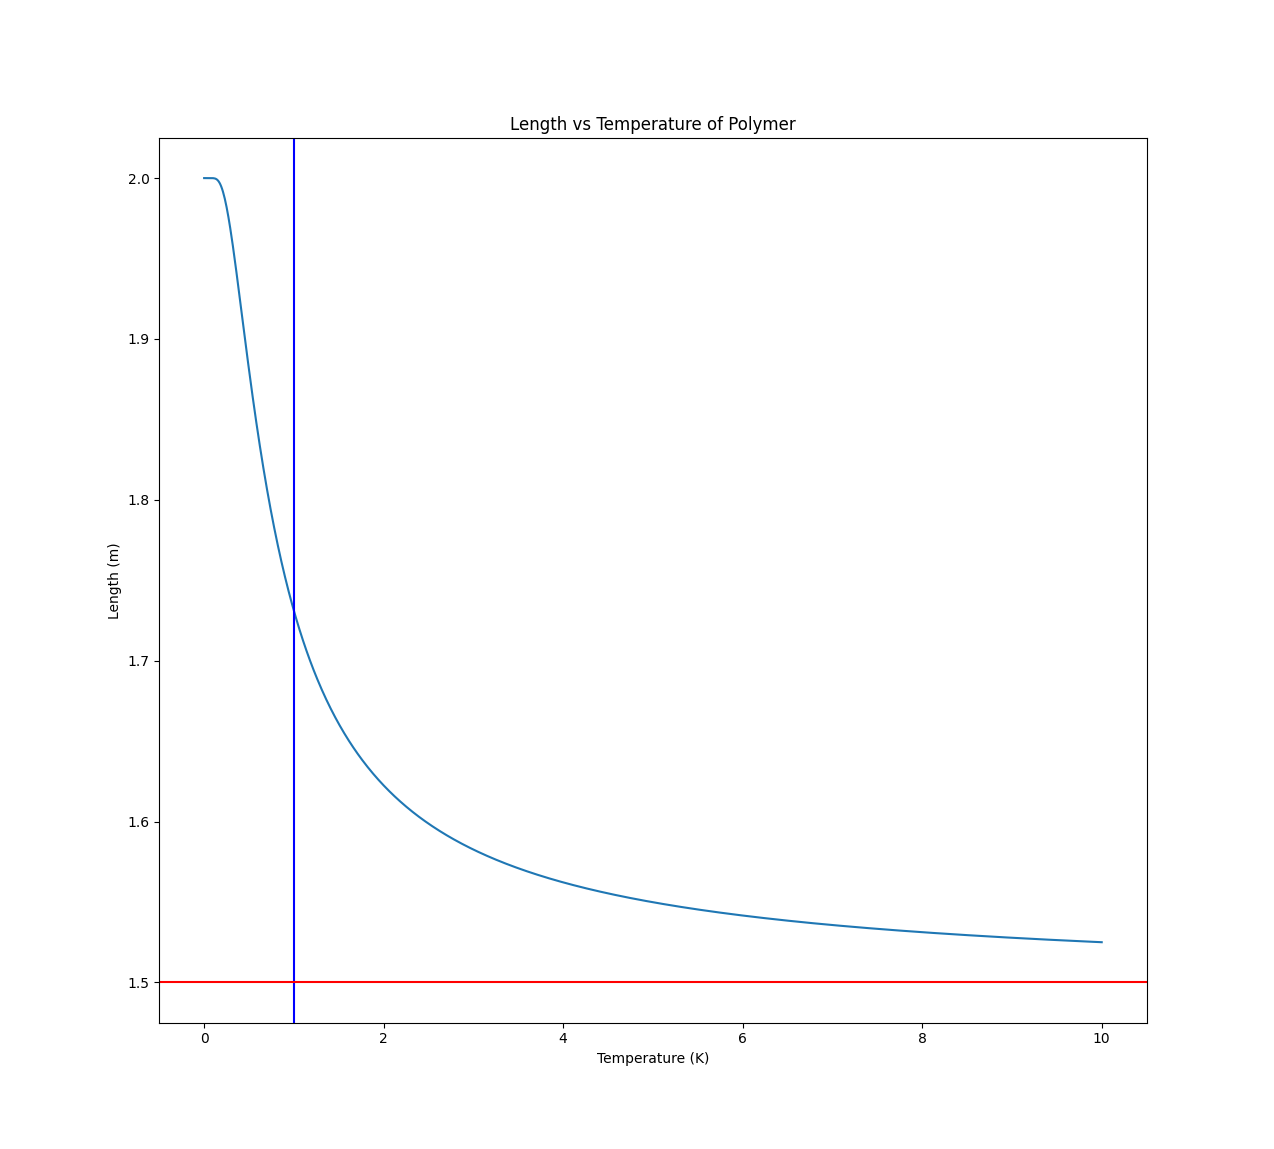
\includegraphics[width=0.8\textwidth]{q4}
    \caption{Graph for question 4. All the physical constants were arbitrarily scaled, see the code for their values. The blue line is when $T= \frac{\epsilon}{k_B}$, which is approximately when the function switches from the flat beginning part to the exponential decay. The red line is at $\frac{N}{2}\left( \ell_l+\ell_s\right) $, which is when maximum entropy is achieved so higher temperatures can't change the length further than this.}
    \label{fig:q4}
\end{figure}

{\medskip\noindent\bf Question II1.} 
\[
\Omega_r(N,V,a)\approx \prod_{j=0}^{N-1}(V-ja)\approx \prod_{j=0}^{N-1}Ve^{-ja /V}=V^{N}e^{-\frac{a}{V}\sum_{j=0}^{N-1}j}=V^{N}e^{-\frac{aN(N-1)}{2V}}
.\]
{\medskip\noindent\bf Question II2.} 
\[
S=k_B\log \Omega(E)=k_B\log\Omega_r(N,V,a)+k_B\log\Omega_p(E)\approx k_B\left( N\log V-\frac{aN(N-1)}{2V}+\frac{3}{2}N\log 2mE \right) 
.\]
\[
T=\left( \frac{\partial S}{\partial E} \right) ^{-1}=\left( \frac{3N}{2E} \right)^{-1}\implies T=\frac{2}{3Nk_B}E\implies E=\frac{3}{2}Nk_BT
.\]
This is the same as for the ideal gas.

{\medskip\noindent\bf Question II3.} The heat capacity is the same as an ideal gas:
\[
C=\frac{dE}{dT}=\frac{3}{2}Nk_B
.\]
For pressure and using that for large $N$ we have $N(N-1)\approx N^2$, we have:
\[
P=T\frac{\partial S}{\partial V}=\frac{k_BTN}{V}+ \frac{k_BTaN(N-1)}{2V^2}\implies (P- \frac{k_BTaN^2}{2V^2})V=Nk_BT
.\]
Qualitatively, this means that for a given volume and temperature the pressure is higher. This makes sense, as compared to an ideal gas, the particles are more restricted in where they can go. Thus they behave as though they were in a slightly smaller volume, which would result in higher pressure.

\end{document}
